\documentclass{article}
\usepackage{soul}
\usepackage[utf8]{inputenc}
\usepackage{xcolor}  % 用于颜色改变
\sethlcolor{yellow}  % 设置highlight的颜色为红色,如果需要黄色则改回yellow
\usepackage{amsmath}
\usepackage{amssymb}
\usepackage{amsfonts}
\usepackage{mathabx}
\usepackage{cancel}
\usepackage{graphicx}
\usepackage{tikz}

\title{MATH2022}
\author{Usyd Mingyuan Ba}
\date{\today}

\begin{document}

\maketitle

\section{Week1}
%================================================================================
\subsection{Arithmetics} % 修正使用 \subsection 或其他适当命令
\begin{itemize}

\item Addition \\
Operations Used: $+,\times$ \\
Limits: $-,/$ 

\item Integers \\
Operations Used: $+,\times,-$ \\
Limits: $/$ 

\item The Rational Numbers  \\
$\mathbb{Q} = \{\frac{p}{q} \mid p,q \in \mathbb{Z}, q \neq 0\}$\\
Operations Used: $+,-,\times,/$ \\
Limits: 

\item The Real Numbers  \\
Operations Used: $+,-,\times,/$ \\
Limits: $i = \sqrt{-1}$ 

\item The Complex Number  \\
$\mathbb{C} = \{a+bi \mid a,b\in \mathbb{R} where i = \sqrt{-1}\}$
Operations Used: $+,-,\times,/$ \\
Limits: 

\item Modular Arithmetic  \\
Let $n \in \mathbb{Z^{*}}$ and let $Z_n$ be the set
of remainders after dividing by n.\\
So $Z_n = \{0,1,2,3 ... n-1\}$

\end{itemize}


%================================================================================
\subsection{Fields}

A \textbf{field} $(F, +, \cdot)$ is a set $F$ equipped with two operations: addition ($+$) and multiplication ($\cdot$), satisfying the following axioms:

\begin{enumerate}
    \item \textit{Closure under Addition and Multiplication}
    \begin{align*}
        \forall a, b \in F, \quad & a + b \in F \\
        \forall a, b \in F, \quad & a \cdot b \in F
    \end{align*}
    
    \item \textit{Associativity of Addition and Multiplication}
    \begin{align*}
        \forall a, b, c \in F, \quad & (a + b) + c = a + (b + c) \\
        \forall a, b, c \in F, \quad & (a \cdot b) \cdot c = a \cdot (b \cdot c)
    \end{align*}
    
    \item \textit{Commutativity of Addition and Multiplication}
    \begin{align*}
        \forall a, b \in F, \quad & a + b = b + a \\
        \forall a, b \in F, \quad & a \cdot b = b \cdot a
    \end{align*}
    
    \item \textit{Identity Elements}
    \begin{align*}
        \exists 0 \in F \, \text{such that} \, \forall a \in F, \quad & a + 0 = a \\
        \exists 1 \in F \, \text{with} \, 1 \neq 0, \, \text{such that} \, \forall a \in F, \quad & a \cdot 1 = a
    \end{align*}
    
    \item \textit{Additive and Multiplicative Inverses}
    \begin{align*}
        \forall a \in F, \quad & \exists -a \in F \, \text{such that} \, a + (-a) = 0 \\
        \forall a \in F \, \text{with} \, a \neq 0, \quad & \exists a^{-1} \in F \, \text{such that} \, a \cdot a^{-1} = 1
    \end{align*}
    
    \item \textit{Distributivity of Multiplication over Addition}
    \begin{align*}
        \forall a, b, c \in F, \quad & a \cdot (b + c) = (a \cdot b) + (a \cdot c)
    \end{align*}
\end{enumerate}

%================================================================================



\subsection{Group Definition}

A \textbf{group} $(G, *)$ is a set $G$ together with a binary operation $*$ that combines any two elements $a$ and $b$ to form another element $a * b$. The binary operation satisfies the following four properties:

\begin{enumerate}
    \item \textit{Closure}: For every $a, b \in G$, the result of the operation $a * b$ is also in $G$.
    \[
    \forall a, b \in G, \quad a * b \in G
    \]

    \item \textit{Associativity}: For every $a, b, and c \in G$, the equation $(a * b) * c = a * (b * c)$ holds.
    \[
    \forall a, b, c \in G, \quad (a * b) * c = a * (b * c)
    \]

    \item\textit{Identity Element}: There exists an element $e \in G$, called the identity element, such that for every element $a \in G$, the equation $e * a = a * e = a$ holds.
    \[
    \exists e \in G \text{ such that } \forall a \in G, \quad e * a = a * e = a
    \]

    \item \textit{Inverse Element}: For each $a \in G$, there exists an element $b \in G$ such that $a * b = b * a = e$, where $e$ is the identity element.
    \[
    \forall a \in G, \quad \exists b \in G \text{ such that } a * b = b * a = e
    \]
\end{enumerate}

A group is called \textbf{abelian} (or \textbf{commutative}) if, in addition, the binary operation is commutative, that is, $a * b = b * a$ for all $a, b \in G$.\\

\textbf{Notes:}
\begin{enumerate}
\item As in the case of fields, the identity element and the inverse can be shown to be unique.
\item Our notation might imply that this operation is multiplication, but it could just as easily be addition or
another operation.
\end{enumerate}


%================================================================================
\subsection{Cyclic Groups}

A \textbf{cyclic group} $G$ is a special type of group that can be entirely generated by a single element $g \in G$. This element $g$ is called a generator of the group. The main characteristic that distinguishes cyclic groups from general groups is the ability to generate all elements of the group by repeatedly applying the group operation to the generator.

\begin{enumerate}
    \item \textit{Generator}
    \begin{align*}
        \exists g \in G \, \text{such that} \, G = \{g^n | n \in \mathbb{Z}\} \, \text{(for multiplicative groups)} \\
        \text{or} \quad G = \{ng | n \in \mathbb{Z}\} \, \text{(for additive groups)}
    \end{align*}
    
    \item \textit{Uniqueness}
    \begin{align*}
        \text{Every element of } G \text{ can be uniquely expressed as } g^n \text{ for some } n \in \mathbb{Z}.
    \end{align*}
\end{enumerate}

The cyclic nature of $G$ implies that it possesses a structure that can be systematically described by the powers (or multiples) of a single element, making cyclic groups particularly simple to understand and work with.

%================================================================================
\newpage
%================================================================================

\subsection{Symmetric Groups}

A \textbf{symmetric group} $S_n$ on a set of $n$ symbols is the group consisting of all possible permutations of these symbols, with group operation being the composition of these permutations. The symmetric group on $n$ symbols is denoted as $S_n$ and plays a crucial role in various areas of mathematics due to its fundamental nature in the study of permutations.\\

\begin{enumerate}
    \item \textbf{Recap}\\
    \textit{definitions}: A bijection is a mapping that is injective (one to one) and surjective (onto). \\

    \hl{\textit{Important Convention}}\\
    We write the action of $f: X \rightarrow Y$ on the right:
    \begin{center}
        $x \mapsto xf$ $(\forall x \in X)$
    \end{center}
    and we compose from left to right:
    \begin{center}
        $fg: X \rightarrow Z$ (where $f:X \rightarrow Y$,
        $g:Y \rightarrow Z$)
    \end{center}
    Instead of using $f \circ g(x) = f(g(x))$, we use $x(fg) := (xf)g$\\
    \textit{We apply f on x first, then g}

    \item Proof that: \textit{The composite of two bijection is also a bijection}\\
    Let $f: X \rightarrow Y, g: Y \rightarrow Z$
    \begin{itemize}
        \item Injective: Need to show that if $x(fg)=y(fg)$ then $x=y$\\
        Suppose $x(fg)=y(fg)$.Then $(xf)g = (yf)g$ by definition,So $xf =yf$ since g is injective,samething agagin, x = y.\\

        \item Surjective: Need to show that the range of $x(fg)$ equals to $Z$
    \end{itemize} 


    \item \textbf{Permutations}
    \begin{itemize}
        \item For a finite set of size n, there are \hl{n!} permutations (write $|X|=n$ ), The set of permutations of X is denoted $Sym(X)$ or $S_x$,So,\hl{$|Sym(X)|=n!$}
    \end{itemize}

    \item \hl{THEOREM}: \\
    The set of permutations on a set X, Sym(X), is a group under composition of permutations. We call it the Symmetric Group on X:

    \begin{itemize}
        \item \textbf{closure} The composite of two bijections is also a bijection.
        \item \textbf{associative} Composition of bijections is associative.
        \item \textbf{Identity element} The identity map is a bijection.
        \item \textbf{Inverse element} The inverse of a bijection is a bijection
    \end{itemize}  


\end{enumerate}

\section{Week2}

\section{Week 3}

\subsection*{Matrix Recap}
\begin{itemize}
    \item \textbf{Elementary Matrices and Invertibility}
    \item \textbf{Determinants, Properties}
\end{itemize}

\subsection*{Odd and Even Permutations}
\begin{itemize}
    \item \textbf{Transposition}\\
    \textit{Definition}: A transposition is a permutation 
    $\phi: \mathbb{X} \rightarrow \mathbb{X}$, which interchanges two distinct elements $a,b \in \mathbb{X}$ leaving all other elements unchanged. Thus,
    \begin{center}
        $\phi = (ab)$.
    \end{center}
    
    \textit{Fact}: All \hl{cycles} are a product (composition) of transpositions.
    \begin{center}
        $(a_1,a_2,a_3, \ldots, a_n) = (a_1 a_2)(a_1a_3)\ldots(a_1a_n)$.
    \end{center}
    
    \textit{Corollary}: Every permutation of a finite set is a product (composition) of transpositions.
    
    \item \textbf{Even/Odd}\\
    \textit{Definition}: We call a permutation even (or odd) if it is a product of an even (or odd, respectively) number of transpositions.
    \begin{itemize}
        \item $(123) = (12)(13)$ is \hl{even}.
        \item $(1234) = (12)(13)(14)$ is \hl{odd}.
        \item $(1) = (12)(12) = (13)(13)$ is \hl{even}.
    \end{itemize}
    \textit{Properties}:
    \begin{itemize}
        \item Single transpositions are self-inverse: $(ab)(ab) = 1$.
        \item A permutation and its inverse have the same parity.
    \end{itemize}


    \item \textbf{Permutation Matrix}\\
    \textit{Definition}: A permutation matrix is the result of applying a permutation to the rows of the identity matrix.
    \begin{center}
        $\phi = (132) = (13)(12) = R_1 \leftrightarrow R_3, R_1 \leftrightarrow R_2$.
    \end{center}
    Hence, \hl{$\text{Det}(M) = \text{Det}(E_1 E_2) = \text{Det}(E_1)\text{Det}(E_2) = (-1)^2 = 1$}.

\end{itemize}
\newpage

\subsection*{The Alternating Subgroup, $\text{Alt}(n)$, of $\text{Sym}(n)$}

\begin{itemize}
    \item \textbf{Subgroup}\\
    \textit{Definition}: A subgroup, $H$, of a group, $G$, is a subset of $G$ which is also a group 
    under the same operation. We write $H \leq G$ or $H < G$ if $H$ is a proper subset of $G$.
    
    \textit{Proof a subgroup}:
    \begin{itemize}
        \item It is non-empty
        \item  It is closed under the operation.\\
        Associativity: Inherited from G\\
        Identity: $\exists a \in G, a^k = e$ \\
        Inverse: $a^k = e \rightarrow aa^{k-1} = e = a^{k-1}a$
    \end{itemize}



    \item \textbf{Alternating Group}\\
    \textit{Definition}: The alternating group (on \(n\) letters) is the set of even permutations 
    in \(Sym(n)\). That is, \(Alt(n) = \{\)even permutations of \(\{1, 2, \ldots, n\}\}\).
    \begin{figure}[htbp]
        \centering % 图片居中
        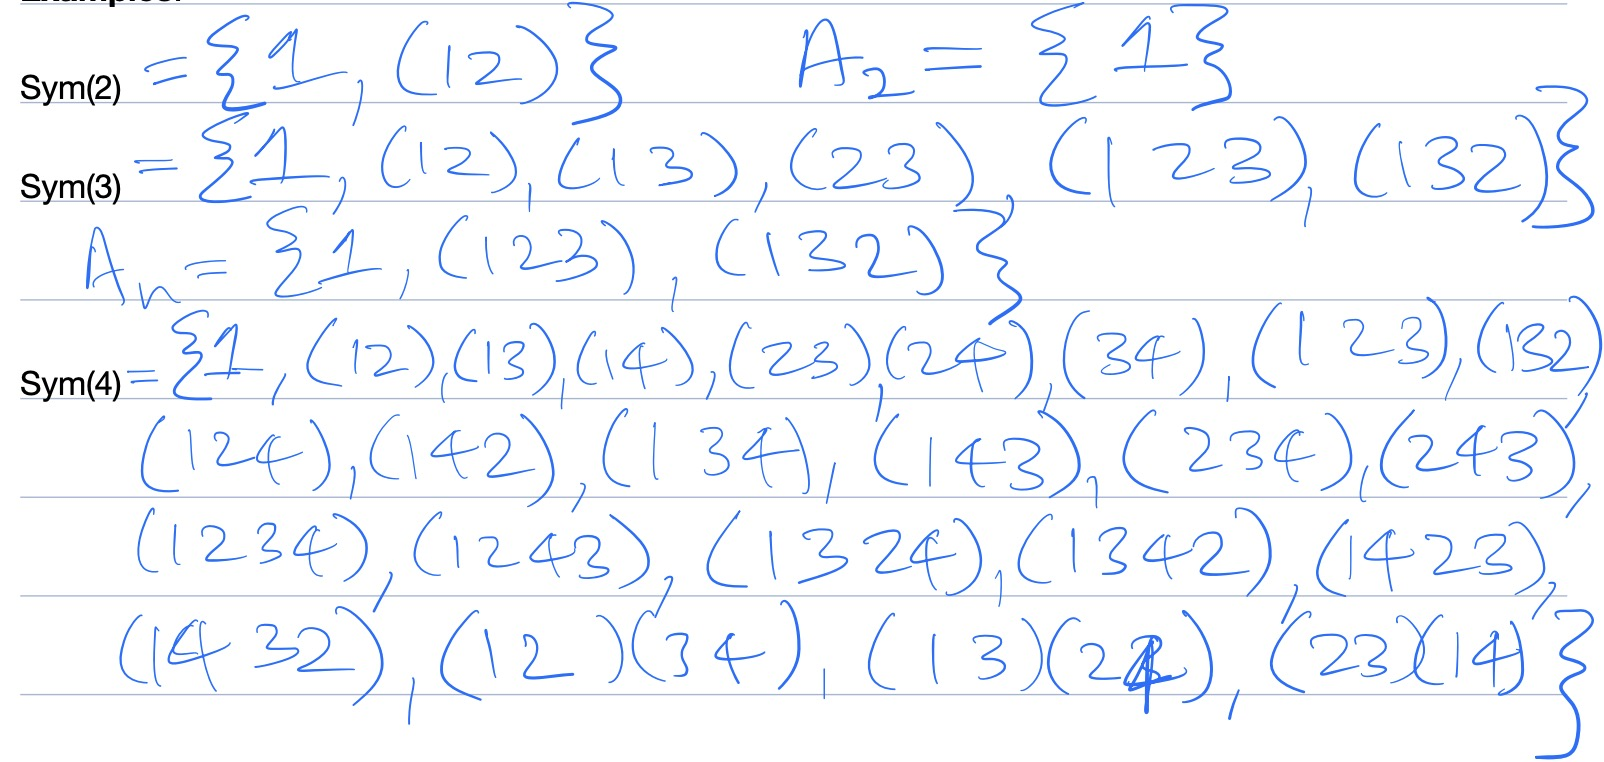
\includegraphics[width=1.0\textwidth]{Graphs/Alternative_Group.jpg} % 插入图片,并设置图片宽度为文本宽度的80%
    \end{figure}

\end{itemize}

\newpage

\section{Week4}

\begin{enumerate}
    \item Elementary matrices: An $n \times n$ matrix is called elementary if it is the result of applying a single elementary row operation to the identity matrix $I_{n}$.
    \item Effect of multiplication by an elementary matrix: If $E$ is the elementary matrix obtained by applying the elementary row operation $\rho$ to $I_{n}$, and $A$ is any matrix with $n$ rows, then the matrix product $E A$ is the matrix obtained by applying $\rho$ to $A$.
    \item Invertibility criterion and algorithm: A square matrix $A$ is invertible if and only if $A$ is a product of elementary matrices, which occurs if and only if the augmented matrix $[A \mid I]$ can be row reduced to $[I \mid B]$, in which case $A^{-1}=B$.
    \item Half of the definition of invertibility suffices for square matrices: If $A$ is a square matrix and $A B=I$ or $B A=I$ then $A B=B A=I$, in which case the inverse $A^{-1}$ exists and equals $B$.
    \item Determinants of matrices of dimensions 1,2 and 3: The determinant of a $1 \times 1$ matrix $[a]$ is simply the entry $a$. The determinant of a $2 \times 2$ matrix $A=\left[\begin{array}{cc}a & b \\ c & d\end{array}\right]$ is $\det A=\left|\begin{array}{cc}a & b \\ c & d\end{array}\right|=a d-b c$. The determinant of a $3 \times 3$ matrix $A=\left[\begin{array}{ccc}a & b & c \\ d & e & f \\ g & h & k\end{array}\right]$ is
    \[
    \det A=|A|=a\left|\begin{array}{cc}
    e & f \\
    h & k
    \end{array}\right|-b\left|\begin{array}{cc}
    d & f \\
    g & k
    \end{array}\right|+c\left|\begin{array}{cc}
    d & e \\
    g & h
    \end{array}\right|
    \]
    called the expansion along the first row, where the smaller determinant arises by ignoring the row and column of the entry being used as a coefficient.
    \item Determinants in general: Following the pattern for $3 \times 3$ matrices, we may expand along any row or down any column of a given square matrix $A$ of any size, producing the same number, called the determinant of $A$, denoted by $\det A$ or $|A|$, provided one uses adjustment factors given by the chequerboard patterns
    \[
    \left[\begin{array}{ccc}
    + & - & + \\
    - & + & - \\
    + & - & +
    \end{array}\right], \quad\left[\begin{array}{cccc}
    + & - & + & - \\
    - & + & - & + \\
    + & - & + & - \\
    - & + & - & +
    \end{array}\right]
    \]
    and so on to higher dimensions.
    \item Multiplicative property of determinants: If $A$ and $B$ are square matrices of the same size then $\det(A B)=(\det A)(\det B)$.
    \item Invertibility criterion using determinants: A square matrix is invertible if and only if its determinant is nonzero.
    \item Effects of elementary row and columns operations on determinants: Let $A$ be a square matrix. If $B$ is obtained from $A$ by swapping two rows or swapping two columns then
    \[
    \det B=-\det A \text{.}
    \]
    If $B$ is obtained from $A$ by multiplying a row or column by a scalar $\lambda$ then
    \[
    \det B=\lambda \det A \text{.}
    \]
    If $B$ is obtained from $A$ by adding a multiple of one row [column] to another row [column] then
    \[
    \det B=\det A \text{.}
    \]
    \item Determinant of the transpose: If $A$ is a square matrix then $\det\left(A^{T}\right)=\det A$.
    \item Transpositions: A permutation that interchanges two letters and fixes all other letters is called a transposition.
    \item \hl{Even and odd permutations:} A permutation of a finite set is called even if it is a product of an even number of transpositions (and by default the identity permutation is even), and called odd if it is a product of an odd number of transpositions.
    \item \hl{No permutation can be both even and odd:} If $n$ is a positive integer then the symmetric group $S_{n}$ is the disjoint union of $A_{n}$, the subset of even permutations (and called the alternating group), and $S_{n} \backslash A_{n}$, the complement of $A_{n}$, which comprises exactly the subset of all odd permutations.
    
    \newpage

    \item \hl{Cosest}:For a Symmetric Group $S_n, n\geq 2$,
    \begin{itemize}
        \item \textbf{Symmetric Group and Cosets:} The symmetric group, denoted as $S_n$, represents the group of all permutations of $n$ elements. Within this group, a \textit{coset} is a form of subset created by multiplying a group element by every element within a subgroup. Specifically, for a subgroup $H$ in a group $G$, and any element $g \in G$, we define:
        \begin{itemize}
            \item A \textit{left coset} of $H$ in $G$ with respect to $g$ as $gH = \{gh : h \in H\}$.
            \item A \textit{right coset} of $H$ in $G$ with respect to $g$ as $Hg = \{hg : h \in H\}$.
        \end{itemize}
        Important properties of cosets include:
        \begin{itemize}
            \item Cosets of a subgroup partition the group.
            \item All left (or right) cosets of a subgroup have the same cardinality as the subgroup itself.
        \end{itemize}
    \end{itemize}

    \begin{figure}[htbp]
        \centering % 图片居中
        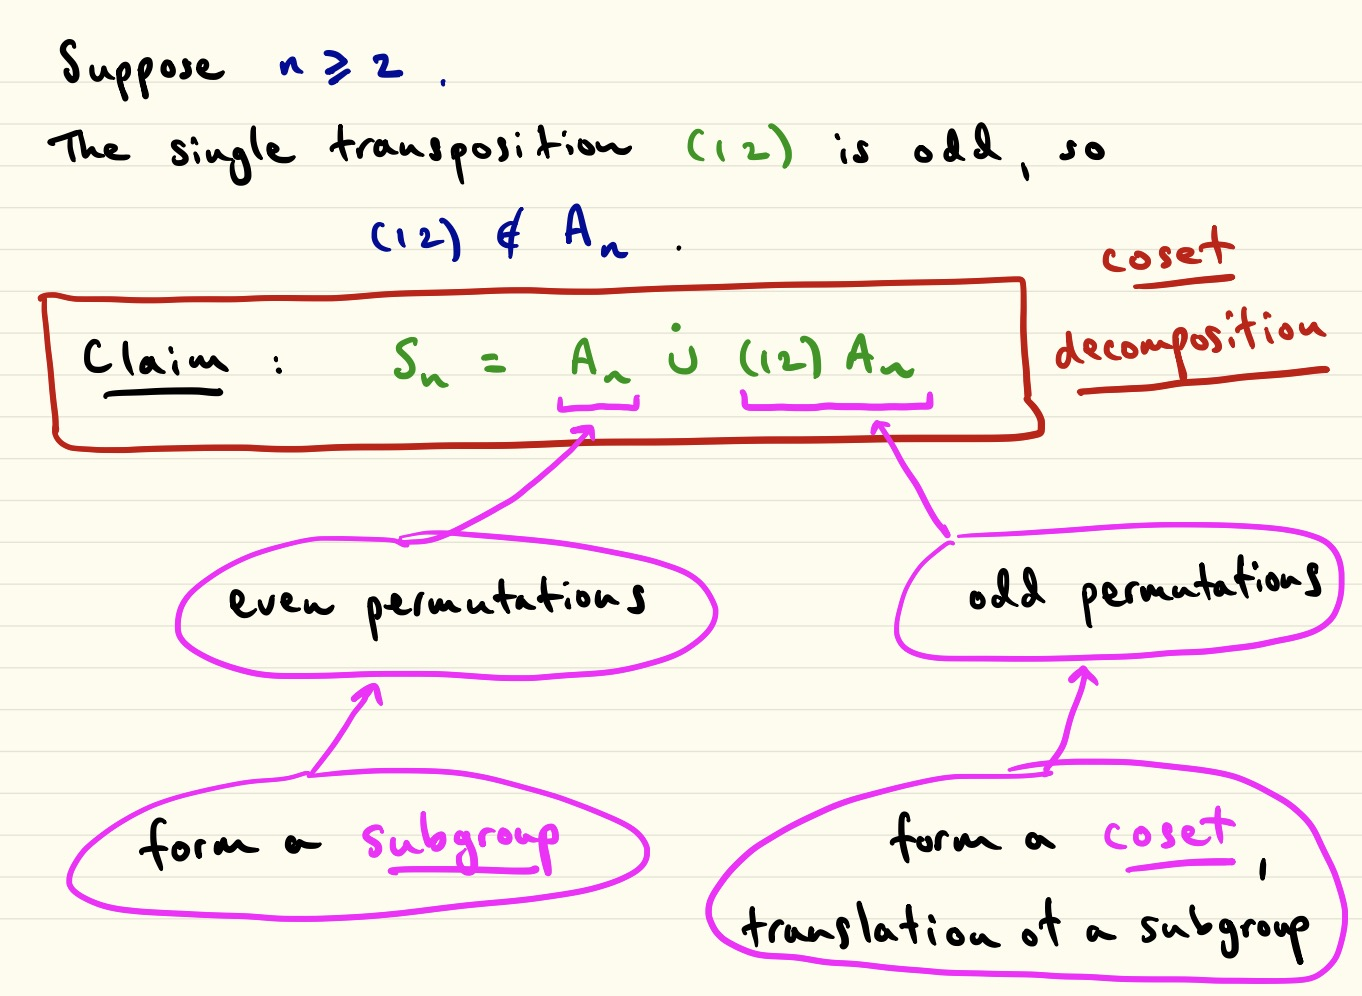
\includegraphics[width=0.8\textwidth]{Graphs/Coset.jpg} % 插入图片,并设置图片宽度为文本宽度的80%
    \end{figure}
    
    \newpage

    \item Conjugates of permutations: If $\alpha$ and $\beta$ are any permutations of a given set then the conjugate of $\alpha$ by $\beta$ is the permutation \hl{$\beta^{-1} \alpha \beta$}, denoted by $\alpha^{\beta}$, using exponential notation. We denote by $\alpha^{-\beta}$ the inverse of $\alpha^{\beta}$, so that $\alpha^{-\beta}=\beta^{-1} \alpha^{-1} \beta$, the conjugate of $\alpha^{-1}$ by $\beta$ (not to be confused with $\beta \alpha \beta^{-1}$, which is $\alpha^{\beta^{-1}}$, the conjugate of $\alpha$ by $\beta^{-1}$.
    \item \textbf{\textit{Properties on Conjugation:}}
            Let $(S,*)$ be a set with an associative binary operation, $*$ , and an identity element, e.
            \begin{itemize}
                \item \textit{multiplicative} $(ab)^c = a^{c}b^{c}$
                \begin{center}
                    $(ab)^c = c^{-1} (a b) c = (c^{-1} a c) (c^{-1} b c) = a^{c}b^{c}$
                \end{center}

                \item $(a^b)^{-1} = (a^{-1})^{b}$ \\
                \textit{Note that}: $a^{b^{-1}}$ is the conjugate of $a$ by $b^{-1}$ 
            \end{itemize}

    \item Effect of conjugation on the cycle decomposition of a permutation: If $\alpha$ and $\beta$ are permutations and $\left(\begin{array}{llll}a_{1} & a_{2} & \ldots & a_{k}\end{array}\right)$ is a cycle in the cycle decomposition of $\alpha$ then $\left(a_{1} \beta a_{2} \beta \ldots a_{k} \beta\right)$ is a cycle in the cycle decomposition of the conjugate $\alpha^{\beta}$.
    \item \textbf{\textit{More on Conjugation}}: \\Suppose $\alpha,\beta \in Sym(n)$,we want to write decomposition of $\alpha^{\beta}$
    from the cycle decomposition of $\alpha$.
    \begin{itemize}
        \item \hl{Lemma}:If $(a_1,a_2,a_3 ...... a_k)$ is cycle in $\alpha$,
        then $(a_1\beta a_2\beta a_3\beta a_4\beta ... a_k\beta)$ is a cycle in $\alpha^{\beta}$.(\hl{$a_k \beta$ means $\beta(a_k)$})
        \\\\\textbf{\textit{Proof}}
        \begin{center}
            Suppose $i \in \{1,2,3 ... k-1\}$,Then\\
            $(a_i \beta) \rightarrow (a_i \beta)(\beta^{-1}a \beta) = a_i \beta \beta^{-1} a \beta
            = a_i a \beta = a_{i+1} \beta$
        \end{center}
        Similarly
        \begin{center}
            $(a_k \beta) \rightarrow (a_k \beta)(\beta^{-1}a \beta) = a_k \beta \beta^{-1} a \beta
            = a_k a \beta = a_1 \beta$
        \end{center}
        \hl{$\rightarrow$} stands for "maps to".
        \\\hl{This proof only shows that the conjugate of a cycle is in(one of) $\alpha^{\beta}$. }
        But in fact:
        \begin{center}
            $(a_1a_2a_3...a_k)^{\beta} = (a_1\beta a_1\beta ... a_k\beta) (\star)$
        \end{center}
        Which means the conjugate of a cycle $a_i$ is exactly a $a_i \beta$.
    \item \textbf{\textit{Corollary}}: To find $\alpha^{\beta}$, just replace every $a_i$, in each cycle with $a_i \beta$
        \begin{center}
            \textbf{Proof}: If $\alpha = a_1 a_2 a_3... a_k$ for cycles $a_i$, 
            the conjugate $\alpha ^{\beta} = a_1 ^{\beta} a_2 ^{\beta} a_2 ^{\beta} ... a_k ^{\beta}$ ------ \textit{multiplicativity}
            \\$= (a_1\beta a_1\beta ... a_k\beta)$ ------ \textit{see $\star$ above}

        \end{center}
    
    \end{itemize}


\end{enumerate}

\section{Week 5}
\begin{enumerate}
    \item Eigenvalues and eigenvectors: Let $M$ be a square matrix, $\mathbf{x}$ a nonzero column vector and $\lambda$ a scalar such that

    $$
    M \mathbf{x}=\lambda \mathrm{x}
    $$

    Then $\lambda$ is called an \hl{eigenvalue} of $M$ and $\mathbf{x}$ is called an \hl{eigenvector} of $M$ associated with or corresponding to the eigenvalue $\lambda$.

    \item The eigenspace of a matrix: The eigenspace of a square matrix $M$ associated with an eigenvalue $\lambda$ is the collection

    $$
    \{\mathbf{v} \mid M \mathbf{v}=\lambda \mathbf{v}\}=\{\mathbf{v} \mid(\lambda I-M) \mathbf{v}=\mathbf{0}\}
    $$

    comprising \hl{all} of the eigenvectors of $M$ associated with $\lambda$ and the zero vector (which is never an eigenvector).

    \item Description of eigenvalues in terms of determinants: A scalar $\lambda$ is an eigenvalue of a square matrix $M$ if and only if

    $$
    \operatorname{det}(\lambda I-M)=0 \text {. }
    $$

    \item The characteristic polynomial of a square matrix: The expression $\operatorname{det}(\lambda I-M)$ is always a polynomial in $\lambda$ and is called the \hl{characteristic polynomial} of $M$. Thus the eigenvalues of a square matrix are precisely the roots of its characteristic polynomial.

    \item Finding eigenspaces: Finding the eigenspace corresponding to the eigenvalue $\lambda$ of a matrix $M$ is equivalent to solving the homogeneous system with coefficient matrix $\lambda I-M$. After the eigenspace has been found, substituting particular values of the parameters yields particular eigenvectors.

    \item Eigenvalues of a triangular matrix: The eigenvalues of a triangular matrix are simply the diagonal entries.

    \item \textit{Notes}:
        \begin{itemize}
            \item Not all real matrices have real Eigenvalues (example later). However, \hl{all complex matrices have complex Eigenvalues}.
        \end{itemize}

    \item The \hl{Cayley-Hamilton Theorem:} Every square matrix $M$ is the root of its own characteristic polynomial, that is,
    $$
    \chi(M)=0
    $$

    where $\chi(\lambda)=\operatorname{det}(\lambda I-M)$ denotes the characteristic polynomial, $\chi(M)$ is the result of evaluating the matrix expression obtained from $\chi(\lambda)$ by substituting $M$ for the indeterminate $\lambda$ and $I$ for the constant 1 , and 0 denotes the zero matrix.\\

    \item Reflection matrices: A reflection matrix in the real plane has the form

    $$
    M=\left[\begin{array}{rr}
    \cos 2 \theta & \sin 2 \theta \\
    \sin 2 \theta & -\cos 2 \theta
    \end{array}\right]
    $$

    for some real $\theta$, and corresponds to reflection in the plane through a line through the origin making an angle $\theta$ with the positive $x$-axis. The eigenvalues of $M$ are $\pm 1$. The eigenspace corresponding to 1 is the line of reflection. The eigenspace corresponding to -1 is the line through the origin perpendicular to the line of reflection.

    \item Rotation matrices: A rotation matrix in the real plane has the form

    $$
    M=\left[\begin{array}{rr}
    \cos \theta & -\sin \theta \\
    \sin \theta & \cos \theta
    \end{array}\right]
    $$

    for some real $\theta$, and corresponds to rotation in the plane anticlockwise through an angle $\theta$ about the origin. The eigenvalues of $M$ are the complex numbers

    $$
    e^{\pm i \theta}=\cos \theta \pm i \sin \theta
    $$

    where $i=\sqrt{-1}$. The eigenvalues are real if and only if $\theta$ is an integer multiple of $\pi$($\sin \theta = 0$), in which case all nonzero vectors are eigenvectors, corresponding to eigenvalue 1 if the integer multiple is even, and corresponding to -1 if the integer multiple is odd.

    \item \textbf{Diagonalization}
    \begin{center}
        $M = PDP^{-1}$
    \end{center}
    Let M be an $n \times n$ Matrix with eigenvalues: $\lambda_1,\lambda_2,\lambda_3...\lambda_n$ (all solutions to chracteristic polynomial $ \chi (\lambda) = det(\lambda) I -M)$),with corresponding eigenvectors $v_1,v_2,v_3,v_4......$(respectively).So that:
    \begin{center}
        $Mv_i = \lambda_i v_i$ for $i = 1, ... n$
    \end{center}
    Let P be the $n \times n$ matrix whose columns are the eigenvectores.So
    \begin{center}
        $P = v_1,v_2,v_3,v_4......v_n$
    \end{center}
    Then $MP = M[v_1,v_2,v_3...v_n] = PD$\\
    \hl{If P is invertible} then we can rearrange to $M = PDP^{-1}$
    We say that M has been diagonalised. Also, M is the conjugate of D by the inverse of P
    Rearranging again, we see that D is the conjugate of M by P: $D = P^{-1}MP$\\

    \textbf{Corollary}
    \begin{center}
        $M^n = P D^n P^{-1}$
    \end{center}


    \item Perron’s Paradox: Let N be the largest positive integer.If $N > 1$, then $N^2 > N$, contradicting the definition of $N$. Hence $N=1$.

    \item \textbf{Perron’s Theorem}: If $M$ is a square matrix with all positive real entries then $M$ has a positive real eigenvalue,$\lambda$, such that $|\mu| < \lambda$ for all eigenvalues $|\mu|$ of $M$. Furthermore, a corresponding eigenvector with only positive entries exists for $\lambda$.We call $\lambda$ the \hl{dominant eigenvalue}.\\

    \textbf{Method}:We can estimate the dominant eigenvalue by iterating powers of $M$ multiplied by a random non-zero vector.
        \begin{enumerate}
            \item choose a starting vector $v_0$
            \item calculate $v_1 = Mv_0$, $v_2 = Mv_1$... , In general $v_{k+1} = Mv_k$
            \item At each step in the process we will “normalise” the vector to make comparisons easier. We repeat until the answers converge.
        \end{enumerate}
\end{enumerate}

\newpage

\section{Week 6}
    \begin{enumerate}
        \item Diagonal matrices: A square matrix $D$ is diagonal if all entries off the diagonal are zero. If $D$ and $E$ are diagonal then $D E=E D$ is also diagonal, and its diagonal entries are simply the products of corresponding diagonal entries of $D$ and $E$. Thus the diagonal elements of $D^{n}$ are just the $n$th powers of the diagonal elements of $D$. A scalar matrix is a diagonal matrix in which all elements along the diagonal are equal. The scalar matrices commute with all square matrices of the same size.

        \item Diagonalisation: Let $M$ be a square $n \times n$ matrix with eigenvalues $\lambda_{1}, \ldots, \lambda_{n}$ and corresponding eigenvectors $\mathbf{v}_{1}, \ldots, \mathbf{v}_{n}$. Then

            $$
            M P=P D
            $$

        where $D$ is the diagonal matrix with eigenvalues down the diagonal and $P$ the matrix with corresponding eigenvectors as columns. \hl{If $P$} is invertible then

            $$
            M=P D P^{-1} \quad \text { and } \quad D=P^{-1} M P
            $$

        In this case we say that $M$ is diagonalisable, in which case powers of $M$ can be found easily by the formula

            $$
            M^{k}=P D^{k} P^{-1} .
            $$

        If the eigenvalues are all different then $P$ is invertible and $M$ is diagonalisable.
        \item \textbf{Terminologies}
            \begin{enumerate}
                \item Doubly stochastic matrix: has both rows and columns adding to 1
                \item Idempotent matrix, is a square matrix satisfying: $A^2 = A$
                    \begin{itemize}
                        \item Idempotent matrices have eigenvalues 0 and 1 only.
                        \item If A is an idempotent matrix, $A^n = A$ for all $n \geq 1$
                    \end{itemize}

            \end{enumerate}

        \item Similar matrices: Two matrices $A$ and $B$ are said to be similar or conjugate if there is an invertible matrix $P$ such that $B=P^{-1} A P$. \hl{Similarity is an equivalence relation (that is, similarity is reflexive, symmetric and transitive)}. \textbf{In particular, a matrix is diagonalisable if and only if it is similar to a diagonal matrix}.

        \item Stochastic matrices: A square matrix $M$ is stochastic if all the entries are nonnegative and the columns add to 1, \hl{and regular if}, further, some positive power of $M$ has all positive entries. A column matrix $\mathbf{v}$ is a probability vector if all of its entries are nonnegative and add to 1, and, further, becomes a steady state vector for $M$ \hl{if $M \mathbf{v}=\mathbf{v}$}.

        \item Existence and uniqueness of a steady state vector: If $M$ is a regular stochastic matrix then there exists a unique steady state vector $\mathbf{v}$ for $M$, in which case, for any probability vector $\mathbf{x}$,

            $$
            \lim _{k \rightarrow \infty} M^{k} \mathbf{x}=\mathbf{v}
            $$

        \item More on stochastic matrix:
            Let A be a stochastic matrix:
            \begin{enumerate}
                \item 1 is an eigenvalue of A,and so A has at least one steady-state probabiliry vector $\textbf{v}$, which is fixed by A.
                    \begin{center}
                        $A\textbf{v} = 1 \textbf{v}$
                    \end{center}

                \item All eigenvalues of A are less then or equal to 1 in magnitude

                \item If A is regular (some power of A has all positive entries), then:
                    \begin{itemize}
                        \item $\textbf{v}$ is unique
                        \item             
                            $$
                            \lim _{n \rightarrow \infty} A^{n} = \begin{bmatrix} \textbf{v} & \textbf{v} & \textbf{v} & \cdots \end{bmatrix}
                            $$

                        \item for any probability vector $\textbf{x}$,
                            $$
                            \lim _{n \rightarrow \infty} A^n \underline{x}=\underline{v}
                            $$

                        \item 1 is the dominant eigenvalue.

                    \end{itemize}
            \end{enumerate}


        \item Perron's Theorem and existence of dominant eigenvalues: If $M$ is a square matrix all of whose entries are positive then $M$ has a positive real eigenvalue $\lambda$ such that $|\mu| \leq \lambda$ for all eigenvalues $\mu$ of $M$, and, furthermore, there exists an eigenvector corresponding to $\lambda$, all of whose entries are positive.

    \end{enumerate}

\section{Week 7}

    \begin{enumerate}
        \item Cartesian products of sets and inherited coordinatewise operations: If $A_{1}, A_{2}, \ldots, A_{n}$ are sets then we may form the Cartesian product

        $$
        A_{1} \times A_{2} \times \ldots \times A_{n}=\left\{\left(a_{1}, a_{2}, \ldots, a_{n}\right) \mid a_{1} \in A_{1}, a_{2} \in A_{2}, \ldots, a_{n} \in A_{n}\right\}
        $$

        which has coordinate-wise operations inherited from $A_{1}, \ldots, A_{n}$, in the case that these have arithmetic operations of the same type (such as addition or multiplication). In particular, if $F$ is a field and $n \geq 1$ then we may form the Cartesian power

        $$
        F^{n}=A_{1} \times \ldots \times A_{n}=\left\{\left(a_{1}, \ldots, a_{n}\right) \mid a_{1}, \ldots, a_{n} \in F\right\}
        $$

        where $A_{1}=\ldots=A_{n}=F$, with coordinatewise addition, multiplication and scalar multiplication. In this case the mapping

        $$
        \left(a_{1}, \ldots, a_{n}\right) \mapsto\left[\begin{array}{c}
        a_{1} \\
        \vdots \\
        a_{n}
        \end{array}\right]
        $$

        is a bijection between $F^{n}$ and the set $V$ of all column vectors over $F$ of length $n$ preserving addition and scalar multiplication. Both $F^{n}$ and $V$ are examples of vector spaces (see later), and the previous statement says that $F^{n}$ and $V$ are vector space isomorphic. We also define $F^{0}=\{0\}$, called the trivial vector space.

        \item Identification of $n$-tuples with row vectors: It is common to make the following identification of an $n$-tuple with the row vector obtained by deleting commas and replacing round brackets with square brackets:

        $$
        \left(a_{1}, a_{2}, \ldots, a_{n}\right) \equiv\left[a_{1} a_{2} \ldots a_{n}\right]
        $$

        and then coordinatewise addition and scalar multiplication of $n$-tuples becomes addition and scalar multiplication of row vectors as $1 \times n$ matrices.

        \item Linear transformations (special case): The Cartesian power $F^{n}$ is the prototype structure for an $n$-dimensional vector space (see later for definitions). A function $L: F^{m} \rightarrow F^{n}$, where $m$ and $n$ are nonnegative integers, is called a linear transformation if $L$ respects coordinatewise addition and scalar multiplication, that is, for all $\mathbf{v}, \mathbf{w} \in F^{m}$ and $\lambda \in F$,

        $$
        L(\mathbf{v}+\mathbf{w})=L(\mathbf{v})+L(\mathbf{w}) \text { and } L(\lambda \mathbf{v})=\lambda L(\mathbf{v})
        $$

        equivalently, for all $\mathbf{v}, \mathbf{w} \in F^{m}$ and $\lambda, \mu \in F$,

        $$
        L(\lambda \mathbf{v}+\mu \mathbf{w})=\lambda L(\mathbf{v})+\mu L(\mathbf{w})
        $$

        and we say that $L$ respects or preserves linear combinations. If $m=n$ then $L$ is called a linear operator. It is traditional to use functional notation for linear transformations and operators and to compose them in the reverse order to which they are written down (from right to left, by contrast with the left to right convention commonly used by algebraists). The composite of linear transformations, when defined, is also a linear transformation.\\

        \item Standard basis: For $1 \leq i \leq n$, let $\mathbf{e}_{i}$ be the $n$-tuple with 0 in each place except for 1 in the $i$ th place. Put $B=\left\{\mathbf{e}_{1}, \ldots, \mathbf{e}_{n}\right\}$, called the standard basis for $F^{n}$. If $\mathbf{v}=\left(v_{1}, \ldots, v_{n}\right) \in F^{n}$ then

        $$
        \mathbf{v}=v_{1} \mathbf{e}_{1}+\ldots+v_{n} \mathbf{e}_{n}
        $$

        so that $B$ has the so-called spanning property. Also $B$ is linearly independent (see later).

        \item Matrix of a linear transformation: Let $L: F^{m} \rightarrow F^{n}$ be a linear transformation and let $B_{m}$ be the standard basis for $F^{m}$. Form the $n \times m$ matrix $M_{L}$ where, for $1 \leq i \leq m$, the $i$ th column of $M_{L}$ is $\left(L\left(\mathbf{e}_{i}\right)\right)^{\top}$, the transpose of the row vector $L\left(\mathbf{e}_{i}\right)$. The action of $L$ on row vectors corresponds to matrix multiplication of column vectors by $M_{L}$ in the following sense:

        $$
        L(\mathbf{v})=\mathbf{w} \text { if and only if } \quad M_{L} \mathbf{v}^{\top}=\mathbf{w}^{\top} .
        $$

        \item Matrix multiplication corresponds to composition of linear transformations: Let $L_{1}: F^{m} \rightarrow$ $F^{n}$ and $L_{2}: F^{n} \rightarrow F^{q}$ be linear transformations, so that $L_{2} L_{1}=L_{2} \circ L_{1}: F^{m} \rightarrow F^{q}$. Then

        $$
        M_{L_{2} L_{1}}=M_{L_{2}} M_{L_{1}}
        $$

        \item Isomorphisms of groups: If $G$ and $H$ are groups then a bijection $\phi: G \rightarrow H$ is called an isomorphism if $\phi$ preserves the group operation, that is, $\left(g_{1} g_{2}\right) \phi=\left(g_{1} \phi\right)\left(g_{2} \phi\right)$ for all $g_{1}, g_{2} \in G$. If there exists an isomorphism between two groups $G$ and $H$ then we say that $G$ and $H$ are isomorphic and write $G \cong H$. Then $\cong$ is an equivalence relation on the class of groups, that is, $\cong$ is reflexive, symmetric and transitive.

        \item Cyclic groups: A group $G$ is called cyclic if there exists an element $g$, called the generator of $G$ such that every element is a power (possibly negative) of $g$ (expressing the group operation multiplicatively). If a cyclic group is finite then every element is a positive power of the chosen generator. Two cyclic groups are isomorphic if and only if they have the same number of elements.

        \item Shear matrices: A (standard) shear matrix is an elementary matrix of the form

        $$
        \left[\begin{array}{ll}
        1 & k \\
        0 & 1
        \end{array}\right]
        $$

        for some real number $k$, which corresponds to the shear transformation of the $x y$-plane that fixes the $x$-axis and shifts points sideways proportional to their $y$-coordinates (with factor $k$ of proportionality).

        \item Invertible linear transformations of the plane: Every invertible linear transformation of the plane decomposes as the composite of a shear, a pair of dilations in the $x$ and $y$-directions respectively and a rotation. Equivalently, every invertible $2 \times 2$ real matrix decomposes as a product of a shear matrix, a diagonal matrix and a rotation matrix.

    \end{enumerate}

\section{Week 8}
    \begin{enumerate}
        \item Abstract vector spaces: Given a fixed field $F$, a vector space over $F$ is an abelian group $V$ with respect to addition, which is compatible with scalar multiplication by elements of $F$ (denoted by juxtaposition), in the following respects:

        $$
        \begin{gathered}
        (\forall \lambda, \mu \in F)(\forall \mathbf{v}, \mathbf{w} \in V) \quad(\lambda+\mu) \mathbf{v}=\lambda \mathbf{v}+\mu \mathbf{v} \quad \text { and } \quad \lambda(\mathbf{v}+\mathbf{w})=\lambda \mathbf{v}+\lambda \mathbf{w} \\
        (\forall \lambda, \mu \in F)(\forall \mathbf{v} \in V) \quad \lambda(\mu \mathbf{v})=(\lambda \mu) \mathbf{v}
        \end{gathered}
        $$

        and

        $$
        (\forall \mathbf{v} \in V) \quad 1 \mathbf{v}=\mathbf{v}
        $$

        Here 1 is the multiplicative identity element of $F$ and the addition symbol + has to be read in context, belonging either to $V$ or to $F$. It is an important theorem that $V$ is isomorphic to $F^{n}$ for some $n$ (where $n$ may be infinite, with an appropriate interpretation).

        \item Vector space isomorphism: A mapping $\phi: V \rightarrow W$, where $V$ and $W$ are vector spaces over a field $F$ is called a vector space isomorphism if it is a bijection that preserves addition and scalar multiplication, that is, $\phi(\mathbf{v}+\mathbf{w})=\phi(\mathbf{v})+\phi(\mathbf{w})$ and $\phi(\lambda \mathbf{v})=\lambda \phi(\mathbf{v})$ for all $\mathbf{v}, \mathbf{w} \in V$ and $\lambda \in F$ (or, equivalently, preserves linear combinations).

        \item Important examples of vector spaces: Let $F$ be a field.
            \begin{itemize}
                \item The trivial vector space is $F^{0}=\{0\}$, consisting of the zero vector with trivial addition and scalar multiplication.

                \item If $n \geq 1$ then $F^{n}$, the Cartesian power, consisting of all $n$-tuples of elements of $F$, forms a vector space with respect to coordinate-wise addition and scalar multiplication. We may identify $n$-tuples with row vectors of length $n$, in which case the vector addition and scalar multiplication of $n$-tuples become addition and scalar multiplication of row matrices.

                \item If $m, n \geq 1$ then the set Mat ${ }_{m, n}$ of all $m \times n$ matrices forms a vector space with respect to matrix addition and scalar multiplication. In particular, Mat ${ }_{1, n}$, the vector space of row matrices, is identified with $F^{n}$. The vector space Mat ${ }_{m, 1}$ of column matrices of length $m$ is isomorphic to $F^{m}$ under the mapping that takes a matrix to its transpose.

                \item If $n \geq 0$ then the set $\mathbb{P}_{n}$ of all polynomials, with coefficients from $F$, of degree at most $n$ forms a vector space with respect to addition of polynomials and multiplication by constants. Then $\mathbb{P}_{n}$ is isomorphic to $F^{n+1}$.

                \item Let $X$ be a nonempty set. Then the set of all functions from $X$ into $F$, denoted by $F^{X}$, forms a vector space with respect to addition of functions and multiplication of a function by a scalar, defined by the following rules, for $f, g \in F^{X}$ and $\lambda \in F$ :

                $$
                (f+g)(x)=f(x)+g(x) \quad \text { and } \quad(\lambda f)(x)=\lambda f(x) \quad \text { for all } x \in X
                $$
            \end{itemize}

        \item Subspaces: A subspace of a vector space $V$ over a field $F$ is a nonempty subset $S$ of $V$ that is closed under vector addition and scalar multiplication, that is, for all $\mathbf{v}, \mathbf{w} \in S$ and $\lambda \in S$,

        $$
        \mathbf{v}+\mathbf{w} \in S \quad \text { and } \quad \lambda \mathbf{v} \in S
        $$

        or, equivalently, $S$ is closed under taking linear combinations, that is,

        $$
        \left(\forall \mathbf{v}_{1}, \mathbf{v}_{2} \in S\right)\left(\forall \lambda_{1}, \lambda_{2} \in F\right) \quad \lambda_{1} \mathbf{v}_{1}+\lambda_{2} \mathbf{v}_{2} \in S
        $$

        A subspace $S$ of a vector space $V$ becomes a vector space in its own right, using the vector space operations of $V$ restricted to $S$.

        \item Intersections of subspaces: Let $V$ be a vector space. The intersection of any collection of subspaces of $V$ is also a subspace of $V$. This implies that if $X$ is any subset of $V$ then there exists a smallest subspace of $V$ containing $X$, denoted by $\langle X\rangle$, and referred to also as the span of $X$ (see more below), namely

        $$
        \langle X\rangle=\bigcap\{S \mid S \text { is a subspace of } V \text { containing } X\}
        $$

        the intersection of all subspaces of $V$ containing $X$.

        \item Linear combinations: For $k \geq 1$, a linear combination of vectors $\mathbf{v}_{1}, \ldots, \mathbf{v}_{k} \in V$ is an expression of the form

        $$
        \lambda_{1} \mathbf{v}_{1}+\lambda_{2} \mathbf{v}_{2}+\ldots+\lambda_{k} \mathbf{v}_{k}
        $$

        for some scalars $\lambda_{1}, \ldots, \lambda_{k}$. If $k=1$ then this is interpreted as a scalar multiple of $\mathbf{v}_{\mathbf{1}}$. Note that since $0 \mathbf{v}=\mathbf{0}$, for any vector $\mathbf{v}$, the zero vector is always a linear combination of any collection of vectors.

        \item The span of a set of vectors: Let $X$ be a subset of a vector space $V$ over a field $F$. The span of $X$, denoted by $\langle X\rangle$ is defined to be $\{\mathbf{0}\}$, the trivial subspace of $V$, if $X=\emptyset$, and otherwise

        $$
        \langle X\rangle=\{\text { all possible linear combinations of finite collections of vectors from } X\}
        $$

        It follows, in both cases, that $\langle X\rangle$ is the smallest subspace of $V$ containing $X$ (see above). If $X=\left\{\mathbf{v}_{1}, \ldots, \mathbf{v}_{k}\right\}$ then

        $$
        \langle X\rangle=\left\{\lambda_{1} \mathbf{v}_{1}+\lambda_{2} \mathbf{v}_{2}+\ldots+\lambda_{k} \mathbf{v}_{k} \mid \lambda_{1}, \ldots, \lambda_{k} \in F\right\}
        $$

        \item Row and column spaces of a matrix: Let $M$ be an $m \times n$ matrix. The row space of $M$ is the vector space of row vectors of length $n$ spanned by the rows of $M$. The column space of $M$ is the vector space of column vectors of length $m$ spanned by the columns of $M$. Two matrices of the same size have the same row [column] space if and only if they are row [column] equivalent, that is, can be obtained from one another by elementary row [column] operations. The nonzero rows of any row echelon form for $M$ span the row space of $M$ (and in fact form a basis, see later). An analogous statement hold for the column space.

        \item Null space of a matrix: Let $M$ be an $m \times n$ matrix over a field $F$. The null space of $M$ may refer either to the vector space

        $$
        \{\text { column vectors } \mathbf{v} \text { of length } n \mid M \mathbf{v}=\mathbf{0}\}
        $$

        or the solution space of the associated homogeneous system of $m$ equations in $n$ variables:

        $$
        \left\{\mathbf{v} \in F^{n} \mid M \mathbf{v}^{\top}=\mathbf{0}\right\}
        $$
    \end{enumerate}

\section{Week9}
    \begin{enumerate}
        \item Linear dependence and independence: Let $V$ be a vector space over a field $F$, and $\mathbf{v}_{1}, \ldots, \mathbf{v}_{k} \in$ $V$ for some $k \geq 1$. We call the vectors $\mathbf{v}_{1}, \ldots, \mathbf{v}_{k}$ and the set $X=\left\{\mathbf{v}_{1}, \ldots, \mathbf{v}_{k}\right\}$ linearly independent if, for all $\lambda_{1}, \ldots, \lambda_{k} \in F$,

        $$
        \lambda_{1} \mathbf{v}_{1}+\ldots+\lambda_{k} \mathbf{v}_{k}=\mathbf{0} \quad \text { implies } \quad \lambda_{1}=\ldots=\lambda_{k}=0
        $$

        equivalently, in the case $k>1$, \textbf{no vector} from $X$ can be expressed as a linear combination of other vectors from $X$. We say that they are linearly dependent otherwise, that is, if $X=\{\mathbf{0}\}$ or at least one vector from $X$ can be expressed as a linear combination of other vectors from $X$. In particular if $\mathbf{0} \in X$, then $X$ is linearly dependent. If $k=1$ then $X$ is linearly independent if and only if $\mathbf{v}_{1}$ is \textbf{nonzero}. If $k=2$ then $X$ is linearly independent if and only if neither of $\mathbf{v}_{1}$ nor $\mathbf{v}_{2}$ is a scalar multiple of the other. The emptyset $\emptyset$ is declared by definition to be \textbf{linearly independent}. If $Y$ is an infinite subset of $V$ then we say that $Y$ is linearly independent if every finite subset is linearly independent, and otherwise linearly dependent.

        \item Basis and dimension of a vector space: A basis for a vector space $V$ is a \hl{linearly independent} subset $B$ that spans $V$. In particular, the empty set is a basis for the trivial vector space. If follows, when $B$ is nonempty, that every vector in $V$ can be expressed \hl{uniquely} (up to the order of the vectors) as a linear combination of elements of $B$. In applications, a basis $B$ is typically a nonempty finite ordered list of vectors (and order is important with respect to building matrices, see later). It is an important theorem that every vector space $V$ has a basis and every basis for $V$ has the \hl{same size} (even when the size is infinite). The size of any basis for $V$ is called the \hl{dimension} of the vector space and denoted by $\operatorname{dim}(V)$. It is another important theorem that every linearly independent subset can be extended to a basis, and every spanning set contains a basis. It follows that, if $V$ is known to be finite dimensional of dimension $n$, then any linearly independent set or any spanning set of size $n$ is automatically a basis for $V$.

        \item Standard bases: Let $F$ be any field. If $n \geq 1$ then the standard basis for $F^{n}$ is

        $$
        B=\left\{\mathbf{e}_{1}, \ldots, \mathbf{e}_{n}\right\}
        $$

        where $\mathbf{e}_{i}=(0, \ldots, 0,1,0 \ldots, 0)$ with $i$ in the $i$ th place, for $i=1, \ldots, n$. In particular, $F^{n}$ has dimension $n$. The empty set $\emptyset$ is the basis for any trivial vector space (such as $F^{0}$ ), so the \hl{dimension of any trivial vector space is zero}. Let $\mathbb{P}_{n}$ denote the vector space of polynomials in $x$ over $F$ of degree at most $n$, where $n \geq 0$. Then the standard basis for $\mathbb{P}_{n}$ is

        $$
        B=\left\{1, x, \ldots, x^{n}\right\}
        $$

        In particular, $\mathbb{P}_{n}$ has dimension $n+1$.\\
        
        \item Coordinates of a vector with respect to a basis: Let $V$ be a vector space over a field $F$ of dimension $n$ and let $B=\left\{\mathbf{b}_{1}, \ldots, \mathbf{b}_{n}\right\}$ be an ordered basis for $V$. Let $\mathbf{v} \in V$. Then there are unique scalars $\lambda_{1}, \ldots, \lambda_{n} \in F$ such that

        $$
        \mathbf{v}=\lambda_{1} \mathbf{b}_{1}+\ldots+\lambda_{n} \mathbf{b}_{n}
        $$

        We define the coordinate vector (coordinates) of $\mathbf{v}$ with respect to $B$ to be the following column vector:

        $$
        [\mathbf{v}]_{B}=\left[\begin{array}{c}
        \lambda_{1} \\
        \vdots \\
        \lambda_{n}
        \end{array}\right]
        $$

        If $V=F^{n}$ and $B$ is the standard basis for $V$ then $[\mathbf{v}]_{B}=\mathbf{v}^{\top}$, for all $\mathbf{v} \in V$.

        \item \hl{Vector spaces with the same dimension are isomorphic}: If $V$ is a vector space over a field $F$ having a basis $B$ with $n \geq 1$ elements, so has dimension $n$, then $V$ is isomorphic to $F^{n}$ under the mapping $\mathbf{v} \mapsto[\mathbf{v}]_{B}^{\top}$ (for $\mathbf{v} \in V$ ), where the row vector $[\mathbf{v}]_{B}^{\top}$ is, as usual, identified with the $n$-tuple in $F^{n}$. Obviously, all trivial vector spaces, that is, vector spaces of dimension zero, are isomorphic to $F^{0}$.

        \item Isomorphic vector spaces have the same dimension: If $V$ and $W$ are isomorphic vector spaces over a field $F$ and $B$ is a basis for $V$, then it follows that the image of $B$ under the isomorphism is a basis for $W$, and so $V$ and $W$ have the same dimension.

        \item \hl{Nonzero rows of a matrix in row echelon form are linearly independent}: The nonzero rows of a matrix $M$ (over a field $F$ ) in row echelon form are linearly independent and therefore form a basis for the row space of any matrix over $F$ that can be row reduced to yield the same nonzero rows as $M$.

        \item Rank of a matrix: It is an important theorem that the row and column spaces of a matrix $M$ have the same dimension, called the rank of $M$, denoted by $\operatorname{rank}(M)$. The rank is the number of nonzero rows when $M$ or $M^{\top}$ is row reduced to row echelon form.

        \item Nullity of a matrix: Let $M$ be an $m \times n$ matrix over a field $F$. Recall that the null space of $M$ may refer either to the vector space

        $$
        \{\text { column vectors } \mathbf{v} \text { of length } n \mid M \mathbf{v}=\mathbf{0}\}
        $$

        or the solution space of the associated homogeneous system of $m$ equations in $n$ variables:

        $$
        \left\{\mathbf{x} \in F^{n} \mid M \mathbf{x}^{\top}=\mathbf{0}\right\}
        $$

        The dimension of the null space is called the nullity of $M$, denoted by nullity $(M)$. The nullity of $M$ is the number of parameters that need to be introduced to yield the solution of the associated homogeneous system of equations.

        \item Rank-Nullity Theorem for matrices: If $M$ is an $m \times n$ matrix then $\operatorname{rank}(M)+\operatorname{nullity}(M)=n$.


        \item \textbf{Relationship between ....}
            \begin{itemize}
                \item $dim(Row(M)) = dim(Col(M)) = rank(M)$
                \item $nollity(M) = dim(Nol(M)) = dim(M^{\perp})$
                \item to compute nollity of $M$, we reduce $M$ to \textbf{RREF}, then count "free variables" = parameters in the solution set

                \item let $M$ be a $n \times m$ matrix:\\
                $rank(M) = dim(Row(M))$\\
                = \#(nonezero rows in echelon form)\\
                = m - \#(free variables) = $m - nollity(M)$
            \end{itemize}
    \end{enumerate}

\section{Week 10}
    \begin{enumerate}
        \item Matrix exponentials: If $M$ is a real square matrix then we may form the matrix exponential

        $$
        e^{M}=I+M+\frac{M^{2}}{2!}+\frac{M^{3}}{3!}+\ldots
        $$

        It is a theorem that the series always converges. If $M$ is a diagonal $n \times n$ matrix with diagonal entries $\lambda_{1}, \ldots, \lambda_{n}$ then $e^{M}$ is also diagonal with diagonal entries $e^{\lambda_{1}}, \ldots, e^{\lambda_{n}}$. If $A, B$ and $P$ are real square matrices of the same size, $P$ invertible, and $B=P^{-1} A P$ then

        $$
        e^{B}=P^{-1} e^{A} P
        $$

        If $A$ and $B$ commute, that is, $A B=B A$, then $e^{A+B}=e^{A} e^{B}$.

        \item Solving systems of differential equations: Suppose that we have $n$ differentiable functions $x_{1}=x_{1}(t), x_{2}=x_{2}(t), \ldots, x_{n}=x_{n}(t)$ of a real variable $t$ that satisfy the following system of differential equations with constant coefficients:

        $$
        \begin{aligned}
        & x_{1}^{\prime}=a_{11} x_{1}+a_{12} x_{2}+\cdots+a_{1 n} x_{n} \\
        & x_{2}^{\prime}=a_{21} x_{1}+a_{22} x_{2}+\cdots+a_{2 n} x_{n}
        \end{aligned}
        $$

        \begin{center}
        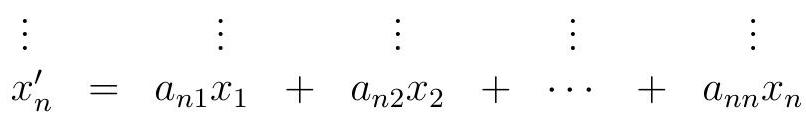
\includegraphics[width=1.0\textwidth]{Graphs/2024_05_26_7d8792d442ce21068082g-1.jpg}
        \end{center}

        Put $\mathbf{x}=\left[\begin{array}{c}x_{1} \\ x_{2} \\ \vdots \\ x_{n}\end{array}\right], \mathbf{x}^{\prime}=\left[\begin{array}{c}x_{1}^{\prime} \\ x_{2}^{\prime} \\ \vdots \\ x_{n}^{\prime}\end{array}\right]$ and $A=\left[\begin{array}{cccc}a_{11} & a_{12} & \ldots & a_{1 n} \\ a_{21} & a_{22} & \ldots & a_{2 n} \\ \vdots & \vdots & \ddots & \vdots \\ a_{n 1} & a_{n 2} & \ldots & a_{n n}\end{array}\right]$, so that the system may

        be expressed in matrix form $\mathbf{x}^{\prime}=A \mathbf{x}$. The solution to this system is

        $$
        \mathbf{x}=e^{t A} \mathbf{c}
        $$

        where $\mathbf{c}=\mathbf{x}(0)$ is a column vector of constants.

        \item Linear transformations (general case): Let $V$ and $W$ be vector spaces over a field $F$. A function $T: V \rightarrow W$ is called a linear transformation if $T$ respects vector addition and scalar multiplication, that is, for all $\mathbf{v}, \mathbf{w} \in V$ and $\lambda \in F$,

        $$
        T(\mathbf{v}+\mathbf{w})=T(\mathbf{v})+T(\mathbf{w}) \quad \text { and } \quad T(\lambda \mathbf{v})=\lambda T(\mathbf{v})
        $$

        or, equivalently, $T$ preserves linear combinations, that is for all $\mathbf{v}_{1}, \mathbf{v}_{2} \in V$ and $\lambda_{1}, \lambda_{2} \in F$,

        $$
        T\left(\lambda_{1} \mathbf{v}_{1}+\lambda_{2} \mathbf{v}_{2}\right)=\lambda_{1} T\left(\mathbf{v}_{1}\right)+\lambda_{2} T\left(\mathbf{v}_{2}\right)
        $$

        If $V=W$ then $T$ is called a linear operator. If $T$ is bijective (one-one and onto) then $T$ is called a vector space isomorphism. The composite of linear transformations, when defined, is also a linear transformation.

        \item  Matrix of a linear transformation with respect to choice of bases: Let $T: V \rightarrow W$ be a linear transformation, and let $B=\left\{\mathbf{b}_{1}, \ldots, \mathbf{b}_{n}\right\}$ and $D=\left\{\mathbf{d}_{1}, \ldots, \mathbf{d}_{m}\right\}$ be ordered bases for $V$ and $W$ respectively. Define the matrix of $T$ with respect to $B$ and $D$ to be

        $$
        [T]_{D}^{B}=\left[\begin{array}{lll}
        {\left[T\left(\mathbf{b}_{1}\right)\right]_{D}} & \cdots & {\left[T\left(\mathbf{b}_{n}\right)\right]_{D}}
        \end{array}\right]
        $$

        by which we mean that we write down, in order, columns of coordinates, in $W$ with respect to $D$, of the images under $T$ of successive basis elements from $B$. Note that $[T]_{D}^{B}$ is an $m \times n$ matrix. It follows from the definitions that, for all $\mathbf{v} \in V$,

        $$
        [T(\mathbf{v})]_{D}=[T]_{D}^{B}[\mathbf{v}]_{B}
        $$

        enabling the effect of the linear transformation $T$ to be described in terms of matrix multiplication between coordinates of vectors. If $S: U \rightarrow V$ is another linear transformation, where $A$ is an ordered basis for $U$, so that $T \circ S: U \rightarrow W$ is also a linear transformation, then

        $$
        [T \circ S]_{D}^{A}=[T]_{D}^{B}[S]_{B}^{A}
        $$

        \item The identity linear operator: Given any vector space $V$ the mapping id $=\mathrm{id}_{V}: V \rightarrow V$ where $\mathrm{id}(\mathbf{v})=\mathbf{v}$, fixing all vectors in $V$, is called the identity linear transformation or identity operator. If $V$ is $n$-dimensional and $B$ is any basis for $V$ then $[\mathrm{id}]_{B}^{B}=I_{n}$, the $n \times n$ identity matrix. If $T: V \rightarrow W$ is a linear transformations then

        $$
        T \circ \mathrm{id}_{V}=T \quad \text { and } \quad \operatorname{id}_{W} \circ T=T
        $$

        Further, if $T$ is a vector space isomorphism, so that $T$ is invertible and $T^{-1}: W \rightarrow V$, then

        $$
        T^{-1} \circ T=\mathrm{id}_{V} \quad \text { and } \quad T \circ T^{-1}=\mathrm{id}_{W}
        $$

        \item Change of basis matrix: Let $B$ and $D$ be any bases for an $n$-dimensional vector space $V$. The matrix $[\mathrm{id}]_{D}^{B}$ is called a change of basis matrix and has the effect of converting coordinates of vectors with respect to $B$ into coordinates with respect to $D$, in the following sense, for any vector $\mathbf{v} \in V$ :

        $$
        [\mathrm{id}]_{D}^{B}[\mathbf{v}]_{B}=[\mathbf{v}]_{D}
        $$

        Furthermore, the change of basis matrices $[\mathrm{id}]_{D}^{B}$ and $[\mathrm{id}]_{B}^{D}$ are mutually inverse, that is,

        $$
        [\mathrm{id}]_{D}^{B}[\mathrm{id}]_{B}^{D}=[\mathrm{id}]_{B}^{D}[\mathrm{id}]_{D}^{B}=I_{n}
        $$
    \end{enumerate}


\end{document}
